\hypertarget{fastaSeqIO_8h}{
\section{Fasta\-Seq\-IO/fasta\-Seq\-IO.h File Reference}
\label{fastaSeqIO_8h}\index{FastaSeqIO/fastaSeqIO.h@{FastaSeqIO/fastaSeqIO.h}}
}
{\tt \#include $<$stdio.h$>$}\par


Include dependency graph for fasta\-Seq\-IO.h:\begin{figure}[H]
\begin{center}
\leavevmode

\includegraphics[width=125pt]{fastaSeqIO_8h__incl}
\end{center}
\end{figure}


This graph shows which files directly or indirectly include this file:\begin{figure}[H]
\begin{center}
\leavevmode
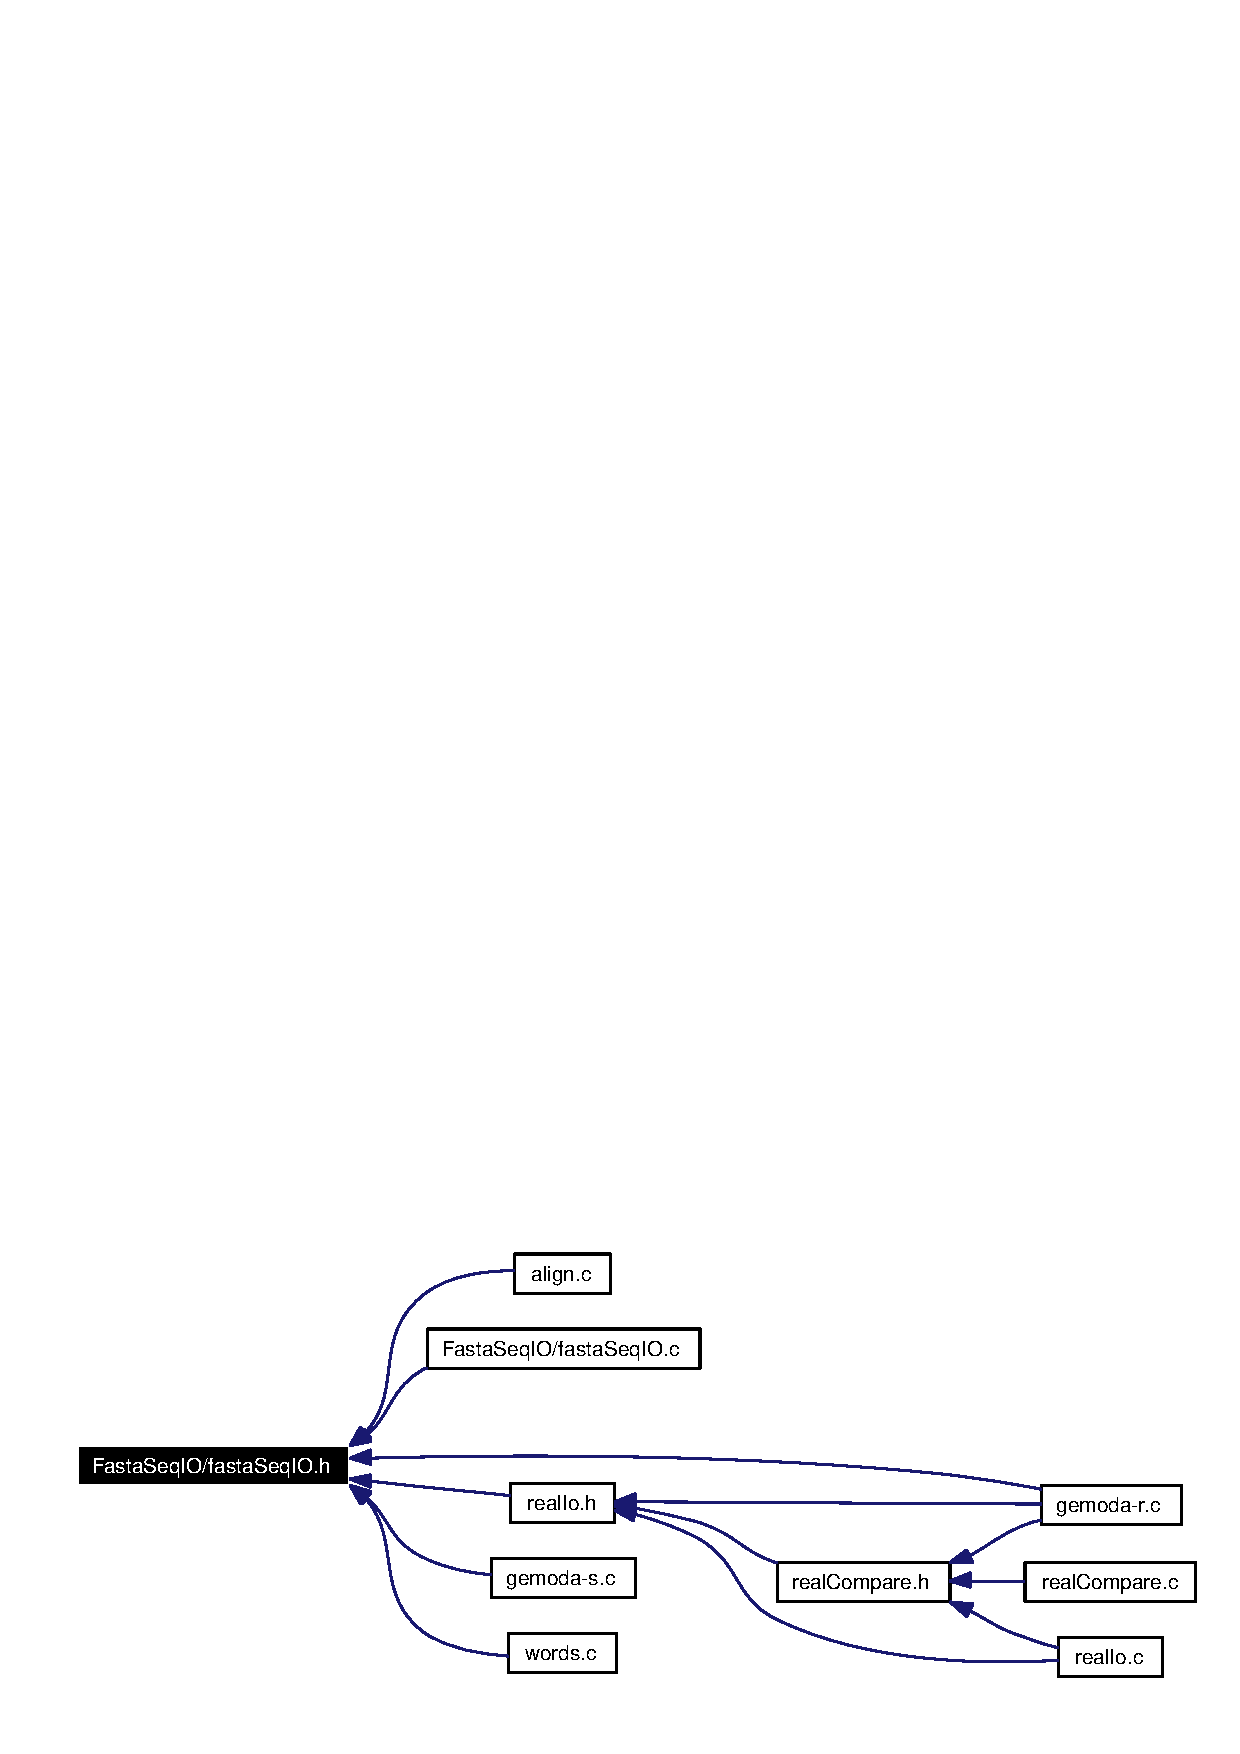
\includegraphics[width=287pt]{fastaSeqIO_8h__dep__incl}
\end{center}
\end{figure}
\subsection*{Data Structures}
\begin{CompactItemize}
\item 
struct \hyperlink{structfSeq__t}{f\-Seq\_\-t}
\end{CompactItemize}
\subsection*{Functions}
\begin{CompactItemize}
\item 
int \hyperlink{fastaSeqIO_8h_a0}{print\-FSeq\-Sub\-Seq} (\hyperlink{structfSeq__t}{f\-Seq\_\-t} $\ast$seq, int start, int stop)
\item 
long \hyperlink{fastaSeqIO_8h_a1}{measure\-Line} (FILE $\ast$INPUT)
\item 
long \hyperlink{fastaSeqIO_8h_a2}{count\-Lines} (FILE $\ast$INPUT)
\item 
long \hyperlink{fastaSeqIO_8h_a3}{Count\-FSeqs} (FILE $\ast$INPUT)
\item 
int \hyperlink{fastaSeqIO_8h_a4}{init\-Aof\-FSeqs} (\hyperlink{structfSeq__t}{f\-Seq\_\-t} $\ast$aos, int num\-Seq)
\item 
\hyperlink{structfSeq__t}{f\-Seq\_\-t} $\ast$ \hyperlink{fastaSeqIO_8h_a5}{Read\-FSeqs} (FILE $\ast$INPUT, int $\ast$number\-Of\-Sequences)
\item 
int \hyperlink{fastaSeqIO_8h_a6}{Free\-FSeqs} (\hyperlink{structfSeq__t}{f\-Seq\_\-t} $\ast$array\-Of\-Sequences, int number\-Of\-Sequences)
\item 
int \hyperlink{fastaSeqIO_8h_a7}{Write\-FSeq\-A} (FILE $\ast$MY\_\-FILE, \hyperlink{structfSeq__t}{f\-Seq\_\-t} $\ast$array\-Of\-Sequences, int start, int stop)
\item 
\hyperlink{structfSeq__t}{f\-Seq\_\-t} $\ast$ \hyperlink{fastaSeqIO_8h_a8}{Read\-Txt\-Seqs} (FILE $\ast$INPUT, int $\ast$number\-Of\-Sequences)
\end{CompactItemize}


\subsection*{Function Documentation}
\hypertarget{fastaSeqIO_8h_a3}{
\index{fastaSeqIO.h@{fasta\-Seq\-IO.h}!CountFSeqs@{CountFSeqs}}
\index{CountFSeqs@{CountFSeqs}!fastaSeqIO.h@{fasta\-Seq\-IO.h}}
\subsubsection[CountFSeqs]{\setlength{\rightskip}{0pt plus 5cm}long Count\-FSeqs (FILE $\ast$ {\em INPUT})}}
\label{fastaSeqIO_8h_a3}




Definition at line 44 of file fasta\-Seq\-IO.c.



\hypertarget{fastaSeqIO_8h_a2}{
\index{fastaSeqIO.h@{fasta\-Seq\-IO.h}!countLines@{countLines}}
\index{countLines@{countLines}!fastaSeqIO.h@{fasta\-Seq\-IO.h}}
\subsubsection[countLines]{\setlength{\rightskip}{0pt plus 5cm}long count\-Lines (FILE $\ast$ {\em INPUT})}}
\label{fastaSeqIO_8h_a2}




Definition at line 69 of file fasta\-Seq\-IO.c.

Referenced by Read\-File().



\hypertarget{fastaSeqIO_8h_a6}{
\index{fastaSeqIO.h@{fasta\-Seq\-IO.h}!FreeFSeqs@{FreeFSeqs}}
\index{FreeFSeqs@{FreeFSeqs}!fastaSeqIO.h@{fasta\-Seq\-IO.h}}
\subsubsection[FreeFSeqs]{\setlength{\rightskip}{0pt plus 5cm}int Free\-FSeqs (\hyperlink{structfSeq__t}{f\-Seq\_\-t} $\ast$ {\em array\-Of\-Sequences}, int {\em number\-Of\-Sequences})}}
\label{fastaSeqIO_8h_a6}




Definition at line 306 of file fasta\-Seq\-IO.c.

References f\-Seq\_\-t::label, and f\-Seq\_\-t::seq.

Referenced by main().



\hypertarget{fastaSeqIO_8h_a4}{
\index{fastaSeqIO.h@{fasta\-Seq\-IO.h}!initAofFSeqs@{initAofFSeqs}}
\index{initAofFSeqs@{initAofFSeqs}!fastaSeqIO.h@{fasta\-Seq\-IO.h}}
\subsubsection[initAofFSeqs]{\setlength{\rightskip}{0pt plus 5cm}int init\-Aof\-FSeqs (\hyperlink{structfSeq__t}{f\-Seq\_\-t} $\ast$ {\em aos}, int {\em num\-Seq})}}
\label{fastaSeqIO_8h_a4}




Definition at line 94 of file fasta\-Seq\-IO.c.

References f\-Seq\_\-t::label, and f\-Seq\_\-t::seq.

Referenced by Read\-FSeqs(), and Read\-Txt\-Seqs().



\hypertarget{fastaSeqIO_8h_a1}{
\index{fastaSeqIO.h@{fasta\-Seq\-IO.h}!measureLine@{measureLine}}
\index{measureLine@{measureLine}!fastaSeqIO.h@{fasta\-Seq\-IO.h}}
\subsubsection[measureLine]{\setlength{\rightskip}{0pt plus 5cm}long measure\-Line (FILE $\ast$ {\em INPUT})}}
\label{fastaSeqIO_8h_a1}




Definition at line 25 of file fasta\-Seq\-IO.c.

Referenced by Read\-File().



\hypertarget{fastaSeqIO_8h_a0}{
\index{fastaSeqIO.h@{fasta\-Seq\-IO.h}!printFSeqSubSeq@{printFSeqSubSeq}}
\index{printFSeqSubSeq@{printFSeqSubSeq}!fastaSeqIO.h@{fasta\-Seq\-IO.h}}
\subsubsection[printFSeqSubSeq]{\setlength{\rightskip}{0pt plus 5cm}int print\-FSeq\-Sub\-Seq (\hyperlink{structfSeq__t}{f\-Seq\_\-t} $\ast$ {\em seq}, int {\em start}, int {\em stop})}}
\label{fastaSeqIO_8h_a0}




Definition at line 14 of file fasta\-Seq\-IO.c.

References f\-Seq\_\-t::seq.



\hypertarget{fastaSeqIO_8h_a5}{
\index{fastaSeqIO.h@{fasta\-Seq\-IO.h}!ReadFSeqs@{ReadFSeqs}}
\index{ReadFSeqs@{ReadFSeqs}!fastaSeqIO.h@{fasta\-Seq\-IO.h}}
\subsubsection[ReadFSeqs]{\setlength{\rightskip}{0pt plus 5cm}\hyperlink{structfSeq__t}{f\-Seq\_\-t}$\ast$ Read\-FSeqs (FILE $\ast$ {\em INPUT}, int $\ast$ {\em number\-Of\-Sequences})}}
\label{fastaSeqIO_8h_a5}




Definition at line 199 of file fasta\-Seq\-IO.c.

References init\-Aof\-FSeqs(), f\-Seq\_\-t::label, Read\-File(), f\-Seq\_\-t::seq, s\-Size\_\-t::size, s\-Size\_\-t::start, and s\-Size\_\-t::stop.

Referenced by main().



\hypertarget{fastaSeqIO_8h_a8}{
\index{fastaSeqIO.h@{fasta\-Seq\-IO.h}!ReadTxtSeqs@{ReadTxtSeqs}}
\index{ReadTxtSeqs@{ReadTxtSeqs}!fastaSeqIO.h@{fasta\-Seq\-IO.h}}
\subsubsection[ReadTxtSeqs]{\setlength{\rightskip}{0pt plus 5cm}\hyperlink{structfSeq__t}{f\-Seq\_\-t}$\ast$ Read\-Txt\-Seqs (FILE $\ast$ {\em INPUT}, int $\ast$ {\em number\-Of\-Sequences})}}
\label{fastaSeqIO_8h_a8}




Definition at line 172 of file fasta\-Seq\-IO.c.

References init\-Aof\-FSeqs(), Read\-File(), and f\-Seq\_\-t::seq.



\hypertarget{fastaSeqIO_8h_a7}{
\index{fastaSeqIO.h@{fasta\-Seq\-IO.h}!WriteFSeqA@{WriteFSeqA}}
\index{WriteFSeqA@{WriteFSeqA}!fastaSeqIO.h@{fasta\-Seq\-IO.h}}
\subsubsection[WriteFSeqA]{\setlength{\rightskip}{0pt plus 5cm}int Write\-FSeq\-A (FILE $\ast$ {\em MY\_\-FILE}, \hyperlink{structfSeq__t}{f\-Seq\_\-t} $\ast$ {\em array\-Of\-Sequences}, int {\em start}, int {\em stop})}}
\label{fastaSeqIO_8h_a7}




Definition at line 332 of file fasta\-Seq\-IO.c.



